\documentclass[10pt]{article}
    \usepackage{listings}
    \usepackage{xcolor}
    \usepackage{graphicx}
    \usepackage{pythonhighlight}
    \usepackage{amsmath}
    \usepackage{subfigure}
    \usepackage[left = 2cm,right = 2cm,top = 3 cm,bottom = 3cm]{geometry}
\lstset{
    numbers = left,
    frame = none,
    backgroundcolor = \color[RGB]{240,244,245},
    keywordstyle = \color[RGB]{0,0,255},
    numberstyle = \footnotesize\color{darkgray},
    commentstyle = \it\color[RGB]{255,96,96},
    stringstyle = \rmfamily\slshape\color[RGB]{255,0,255},
    showstringspaces = false,
    language=C++,
}

\begin{document}
    \title{Study Report}
    \author{Shuo Xu}
    \maketitle
    \begin{abstract}
        Briefly describe the problems I've encountered and the solutions I've come up with. And the leetcode.
    \end{abstract}

    \begin{center}
        \section*{New Problems with CNN}
    \end{center}
    \begin{flushleft}
        After I asked you thats problems, I simplified my code and decided to run it through the 60,000 photos. I set the learning rate to 0.01 and set the batch size to 64. In the process of running the program I found that training a batch of data actually need three seconds. I've simplified the program as much as I can, but the time is still huge.\vspace{2ex}

        After running the program for half an hour, I realized that the batch success rate was below 0.2, and I realised there was a problem inside the program. At first I thought it was my learning rate set is not reasonable enough, so I changed the learning rate and run the program several times. But things aren't getting any better.\vspace{2ex}

        Then I ran the program two times and recorded the initial output.

        \begin{center}
            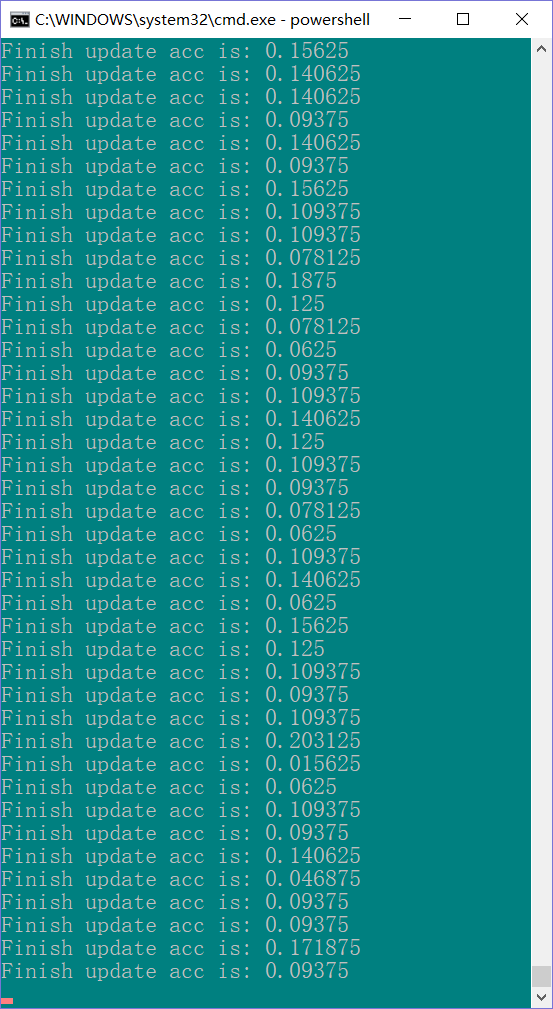
\includegraphics[scale = 0.3]{data1.png}
        \end{center}

        Although the learning rate is different, but each time the output is the same as the picture. So I checked the back-propagation part and found that the gradient disappeared. The calculated derivatives were generally less than 0.1. This is a question that should be first thought of. I am  looking for suitable initialization mode. \vspace{2ex}

        This week I'm also working on improving my code, using classes to write every layer of the neural network, trying to write the form of a tensorflow framework. But the problem of gradient disappearing is still waiting for me to solve.

    \end{flushleft}

    \begin{center}
        \section*{Leetcode}
    \end{center}
    \subsection*{Word Pattern}
    \begin{itemize}
        \item Describtion
        \begin{flushleft}
            Given a pattern and a string str, find if str follows the same pattern.

            Here follow means a full match, such that there is a bijection between a letter in pattern and a non-empty word in str.
        \end{flushleft}

        \item Solution
        \begin{flushleft}
            At first, use istringstream to create a vector from the input str. Use .size() to get the number of the input pattern and the vector we have created. If they are not equal, return false. Then use two map for the next step, the first one is char corresponds to string another one is string corresponds to char. Use a index i to traverse the string and the vector. When meet new elements, use the find function with the two new elements as the keys and end function of map to judge whether elements are stored. If they are not stored, add them to the map. If they are stored, judge whether the values of two map correspond to each other. If not, return false. There is another special case, only one element was stored. In this case, we only need to return false.
        \end{flushleft}

        \item Code
        \begin{lstlisting}
class Solution {
public:
	bool wordPattern(string pattern, string str) {
		istringstream iss(str);
		istream_iterator<string> Itbegin = istream_iterator<string>(iss);
		istream_iterator<string> Itend = istream_iterator<string>();
		vector<string> strs(Itbegin, Itend);
		int len1 = pattern.size(), len2 = strs.size();
		if(len1 != len2)
		return false;
		map<char, string> mp1;
		map<string, char> mp2;
		for(int i = 0; i < len1; i++){
				auto it1 = mp1.find(pattern[i]);
				auto it2 = mp2.find(strs[i]);
				if(it1 == mp1.end() && it2 == mp2.end()){
						mp1[pattern[i]] = strs[i];
						mp2[strs[i]] = pattern[i];
					}
				else if(it1 != mp1.end() && it2 != mp2.end()){
						if(mp1[pattern[i]] != strs[i] || mp2[strs[i]] !=pattern[i])
						return false;
					}
				else
				return false;
			}
		return true;
	}
};
        \end{lstlisting}
    \end{itemize}
\end{document}
